%%%%%%%%%%%%%%%%%%%%%%%%%%%%%%%%%%%%%%%%%%%%%%%%%%%%%%%%%
%                                                       %
%           Validation Sheet of Code_Saturne            %
%                      HERCULE                          %
%                                                       %
%%%%%%%%%%%%%%%%%%%%%%%%%%%%%%%%%%%%%%%%%%%%%%%%%%%%%%%%%

% -------------------------------
% DEFINITION OF PRACTICAL LENGTHS
% -------------------------------
\newlength{\largfigpp}
\setlength{\largfigpp}{4.5cm}
\newlength{\largfigk}
\setlength{\largfigk}{6.5cm}
\newlength{\largfigp}
\setlength{\largfigp}{8cm}
\newlength{\largfign}
\setlength{\largfign}{10cm}
\newlength{\largfigm}
\setlength{\largfigm}{12cm}
\newlength{\largfigt}
\setlength{\largfigt}{13cm}
\newlength{\largfigi}
\setlength{\largfigi}{14cm}
\newlength{\largfigg}
\setlength{\largfigg}{16cm}
\newlength{\largleg}
\setlength{\largleg}{12cm}

\renewcommand{\IMAGES}{./IMAGES}

\chapter{HERCULE Test Bench - Confined Two-phase Gas-Solid Flow}

\sousti{N. Picard - A. Douce (2004), RENUDA}{22/06/2020}
\keywords{Lagrangian Two-Phase, Turbulent ($R_{ij}-\varepsilon~SSG$), two-way coupling, 2D axisymmetric, Langevin approach.}

\section{Test Case Description}

\subsection{Purpose}

The test case relates to two-phase flow of air with co-flowing particles in a configuration which is similar to those found in burners. A recirculation zone is created, which implies that gas-particles interaction happens both in the case where they both flow in the same direction and where they flow in opposite directions. The dispersed phase is poly-disperse. The particle loading is such that particles modify the air flow.

\subsection{Setup Description}


The geometry is presented in figure \ref{schema} and the flow is visualised in figure \ref{ecoulement}.

\noindent
At the primary inlet, air and particles (glass spheres) are injected in the centre of the vertical, cylindrical pipe of length $1,5~m$ and radius $R_2~=~0,15~m$. Air is also injected in the annular, secondary inlet. The primary inlet has a radius of $R_j~=~0,01~m$.

\noindent
Several experimental cases are available (\cite{Rap3} and
\cite{TheseNC}). Amongst those, the case with a mass fraction of 22 \%\footnote{The thesis \cite{TheseNC} also mentions cases with 11\% and 110\% mass loadings} has been selected for the simulations. Experimental data is available along the centre line and at different horizontal plane sections: $z = 0,003~m$,
$z = 0,08~m$, $z = 0,16~m$, $z = 0,24~m$, $z = 0,32~m$, $z = 0,42~m$.


\begin{figure}[H]
   \centerline{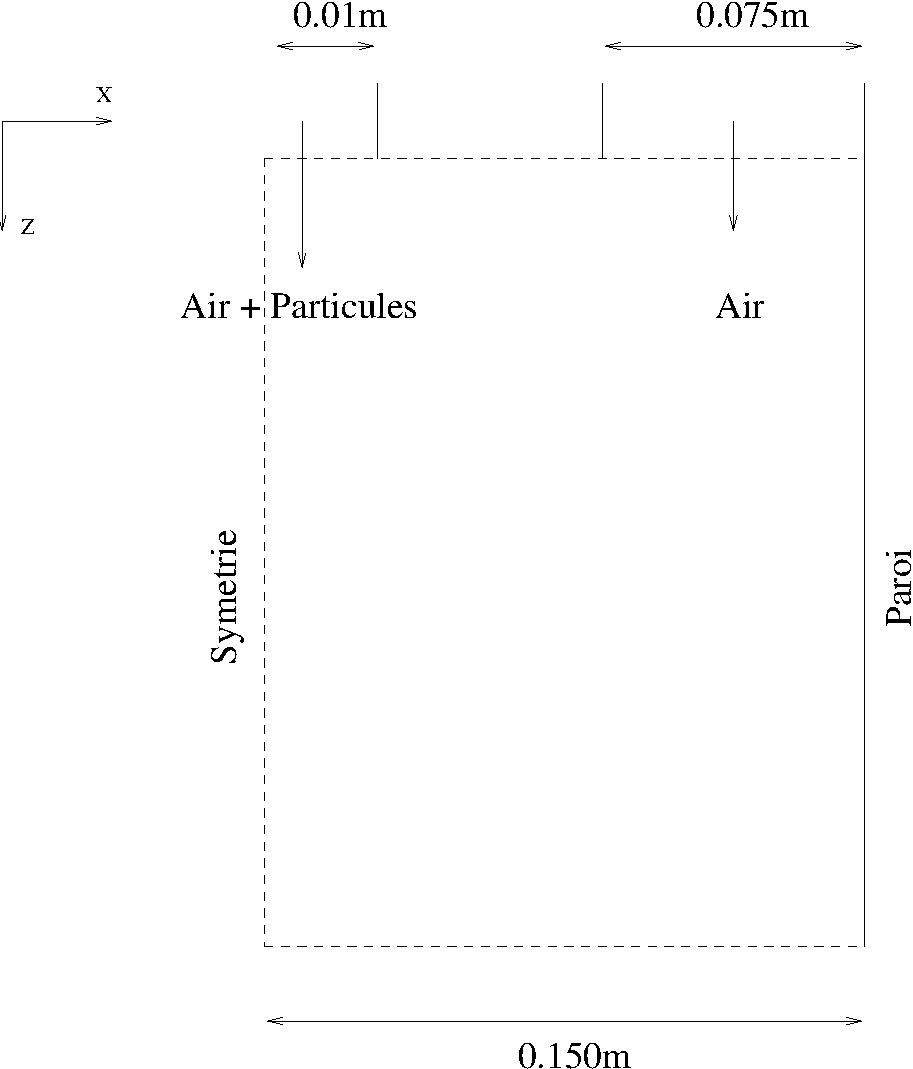
\includegraphics[width={\largfigk}]{\IMAGES/schema.pdf}}
   \caption{Test case geometry.}
   \label{schema}
\end{figure}

\begin{figure}[H]
   \centerline{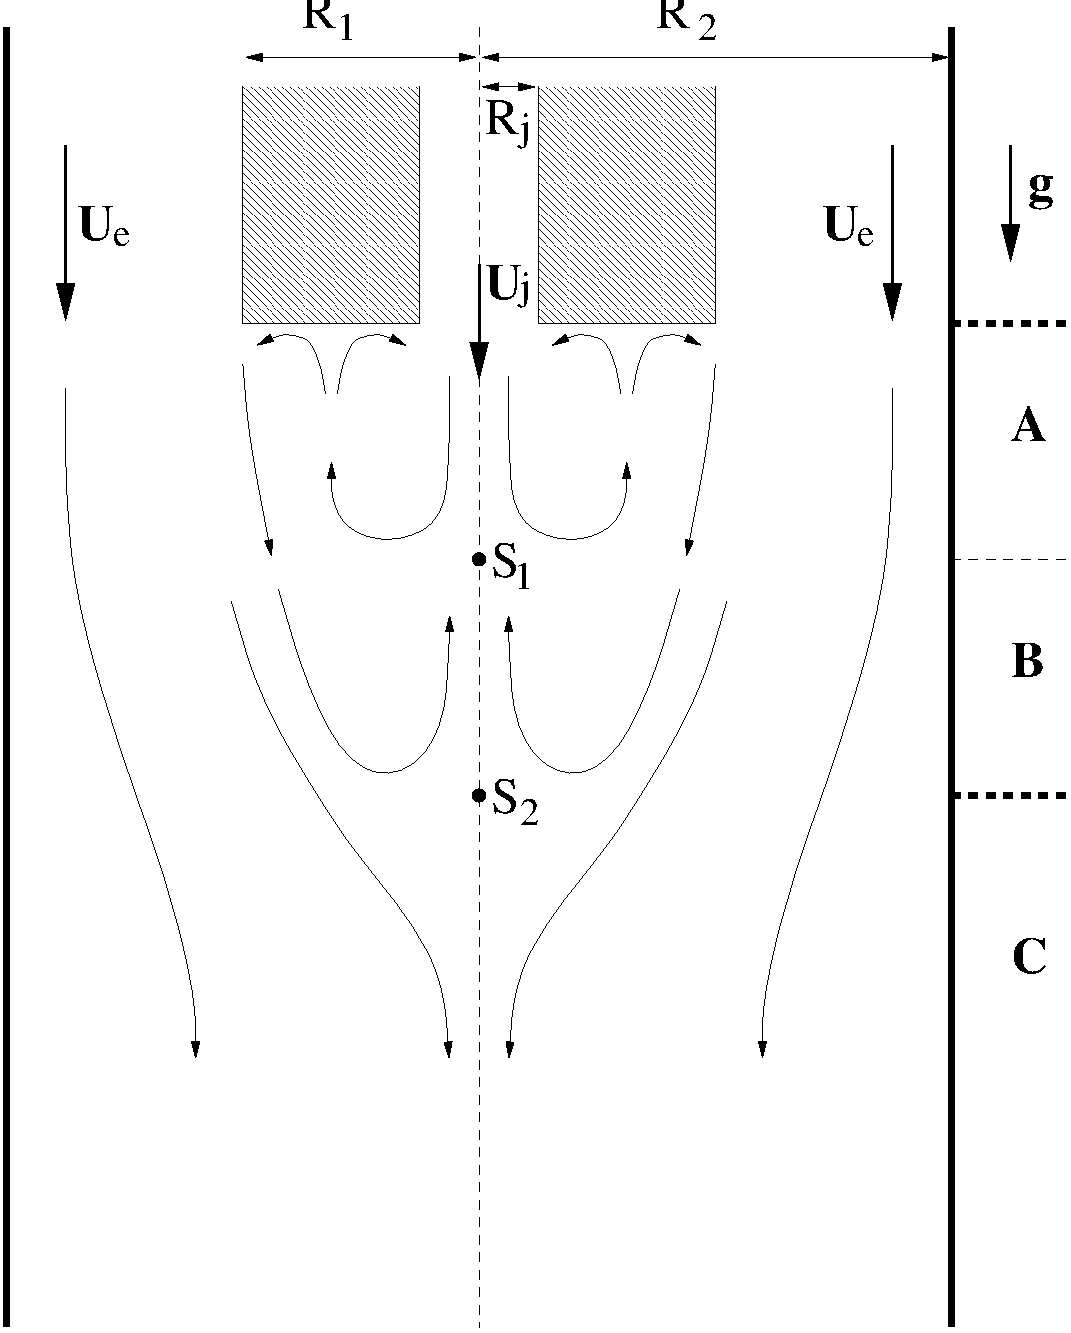
\includegraphics[width={\largfigk}]{\IMAGES/ecoulement-eps-converted-to.pdf}}
   \caption{HERCULE experiment flow schematic.}
   \label{ecoulement}
\end{figure}

\clearpage

\subsection{Test Data}

\begin{itemize}

   \item[$\bullet$] Geometry and operating conditions:

         \begin{table}[!bth]
            \begin{center}
               \begin{tabular}{|l|c|} \hline
                  Pipe diameter              & $0,3~m $ \\ \hline
                  Pipe length                & $1,50~m$ \\ \hline
                  Jet diameter               & $0,02~m$ \\ \hline
                  Jet maximum speed          & $4 ~m/s$ \\ \hline
                  Peripheral injection speed & $6 ~m/s$ \\ \hline
                  Jet Reynolds number        & $3000$   \\ \hline
               \end{tabular}
            \end{center}
         \end{table}

   \item[$\bullet$] Fluid properties

         \begin{itemize}
            \item[-] dynamic viscosity: $\mu~=~1,83337.10^{-5}~kg.m^{-1}.s^{-1}$
            \item[-] density: $\rho~=~1,17861~kg/m^3$
         \end{itemize}
         \vspace{5mm}

   \item[$\bullet$] Particles properties (glass spheres):

         \begin{table}[!bth]
            \begin{center}
               \begin{tabular}{|l|c|} \hline
                  Mean diameter $d_p^{\mu}$       & \  $60~ \mu m$   \\ \hline
                  Standard deviation $\sigma_{p}$ & $14,55 ~\mu m$   \\ \hline
                  Density $\rho_{p}$              & $2470 ~kg/m^{3}$ \\ \hline
                  Mass loading $\phi$             & $0,22$           \\ \hline
               \end{tabular}
            \end{center}
         \end{table}

         \noindent
         The diameter of the particles, $d_p$, is computed based on the mean diameter and the standard deviation using the formula, $d_p = d_p^\mu + \xi \sigma_{p}$, where $\xi$ is a random, non-imaginary variable following a normal law.

\end{itemize}

\subsection{References}

\begin{thebibliography}{3}


   \bibitem{Rap1} J.P. Minier, M. Ouraou, 'Module diphasique Lagrangien
   du code ESTET : calculs de validation et applications industrielles',
   {\it Rapport EDF}, HI-81/01/027/A 2001.

   \bibitem{Rap2} M. Ouraou, J.P. Minier, 'Mod\'elisation Lagrangienne des
   \'ecoulements diphasiques : prise en compte de l'influence des particules
   sur le fluide dans le module d'ESTET',
   {\it Rapport EDF}, HE-44/95/031/A 1995.

   \bibitem{Rap3}  C. Vit, 'Mod\'elisation eul\'erienne d'\'ecoulements
   turbulents diphasiques gaz-solides pr\'esentant une granulom\'etrie
   \'etendue de la phase dispers\'ee.'
   {\it Rapport EDF}, HE-44/99/017/A 1999.

   \bibitem{RefB-6} J.P Minier, E. Peirano,
   ' The PDF approach to turbulent polydispersed two-phase flows'
   {\it Physics Reports}, Vol. 352/1-3, pp. 1-214, September 2001
   (Rapport EDF HI-81/01/025/A, 2001).

   \bibitem{Poz_98} J. Pozorski, J-P. Minier,
   'On the lagrangian turbulent dispersion models based on the langevin
   equation.'
   {\it Int. J. Multiphase Flow}, 24:913--945, 1998.

   \bibitem{Poz_99} J. Pozorski, J-P. Minier,
   'Probability density function modelling of dispersed two-phase
   turbulent flows.'
   {\it Physical Review E}, 59(1):855--863, 1998.

   \bibitem{Min_99} J-P. Minier,
   'Closure proposals for the langevin equation model in {L}agrangian
   two-phase flow modelling.'
   {\it Proceedings of the 3rd ASME/JSME Conference}, pages
   FEDSM99--7885, San Francisco, July 28-23 1999. ASME FED.

   \bibitem{RefB-3} J.P. Minier, J. Pozorski,
   'Analysis of existing Lagrangian models and new
   proposition for particule dispersion in
   homogeneous stationary turbulence.'
   {\it Rapport EDF} HE-44/92.29, 1992.

   \bibitem{TheseNC} N. Caraman,
   'Exp\'erimentation mod\`ele en \'ecoulement gaz-solide co-courant confin\'e.
   Application de la mod\'elisation eul\'erienne \`a l'analyse de l'influence
   du chargement en situation monodispers\'ee ou polydispers\'ee.'
   {\it Rapport EDF} HI-81/01/09/A, 2004.

   \bibitem{RefB-4} A. Douce, J.P. Minier,
   'Mod\'elisation stochastique lagrangienne d'\'ecoulements turbulents
   diphasiques dans \CS'
   {\it Rapport EDF} HI-81/04/03, 2004.

\end{thebibliography}

% =============================
\section{Numerical setup}
% =============================

\subsection{Numerical modelling}

\begin{itemize}

   \item \textbf{Type of calculation} :
         \begin{itemize}
            \item[$\rightarrow$] Continuous phase: incompressible, turbulent, 2D axisymmetric, isothermal.
            \item[$\rightarrow$] Dispersed phase: solid particles, two-way coupling with the complete model with the local rotation option.
            \item[$\rightarrow$] Fluid particles: Langevin approach.
         \end{itemize}

   \item \textbf{Gravity}: Activated

   \item \textbf{Turbulence model}: $R_{ij}-\varepsilon~SSG$

\end{itemize}

\subsection{Mesh}

The mesh represents a 5\textdegree\  wedge. It is made of a single layer containing 8664 mesh cells. The origin is situated on the axis of revolution, in the inlet plane. The whole mesh and details of the mesh are shown in figure \ref{maillage}.

\begin{description}

   \item[\textbf{Type} :] Unstructured, hexahedral mesh with prismatic cells along the centre line.

   \item[\textbf{Coordinate system}:] Cartesian\footnote{In the experiments, the measurements are done in a cylindrical system of coordinates. Therefore the data points must be converted to the mesh coordinate system (user codes cs\_user\_modules.f90,
            cs\_user\_lagr\_particle.c and cs\_user\_boundary\_conditions.f90).}.

   \item[\textbf{Number of cells} :] 8~664

   \item[\textbf{Mesh construction methodology}:] SIMAIL mesher.


\end{description}

\begin{figure}[H]
   \centerline{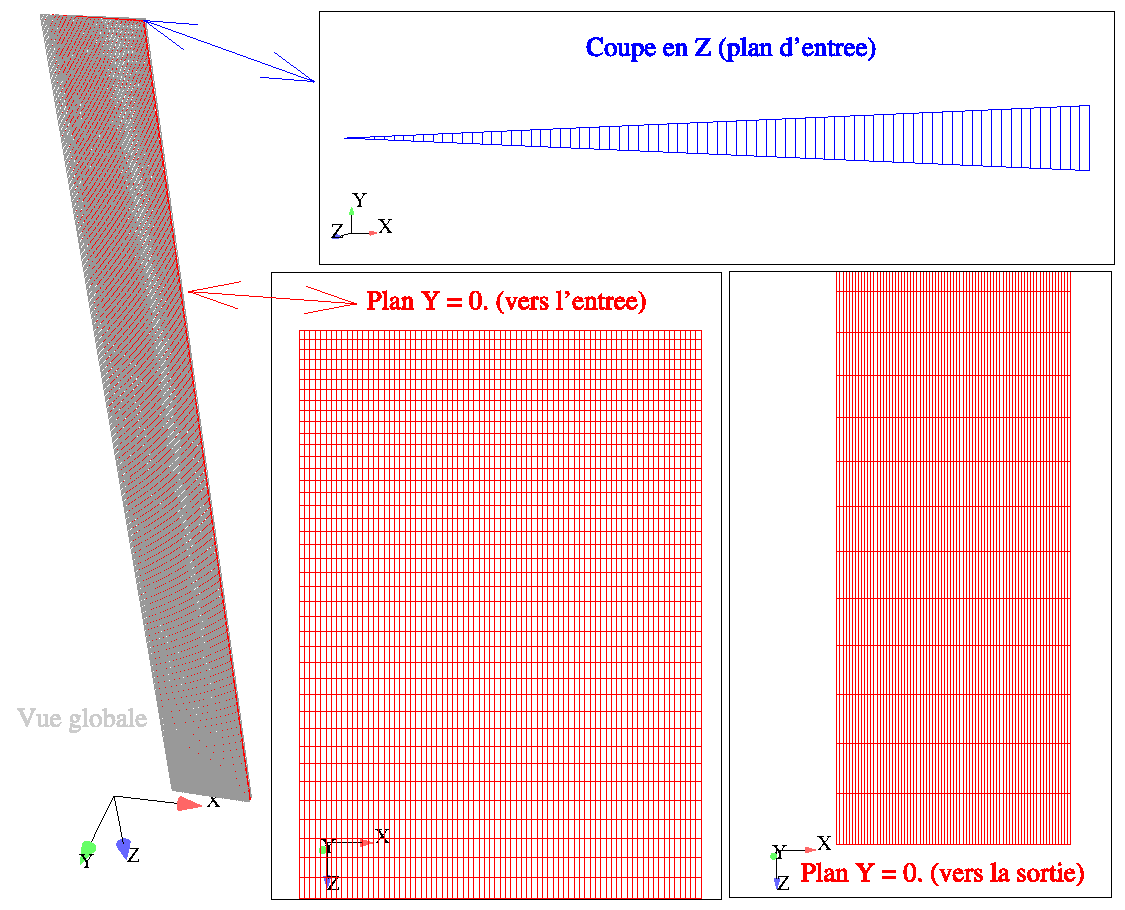
\includegraphics[width=14cm]{\IMAGES/maillage-eps-converted-to.pdf}}
   \caption{\label{maillage}{Mesh}}
\end{figure}

\subsection{Boundary and Initial Conditions}

\begin{itemize}

\item[$\bullet$] \textbf{Specification of the boundary conditions}:

The names of the different boundary conditions are shown in figure \ref{couleur}.

\begin{figure}[H]
   \centerline{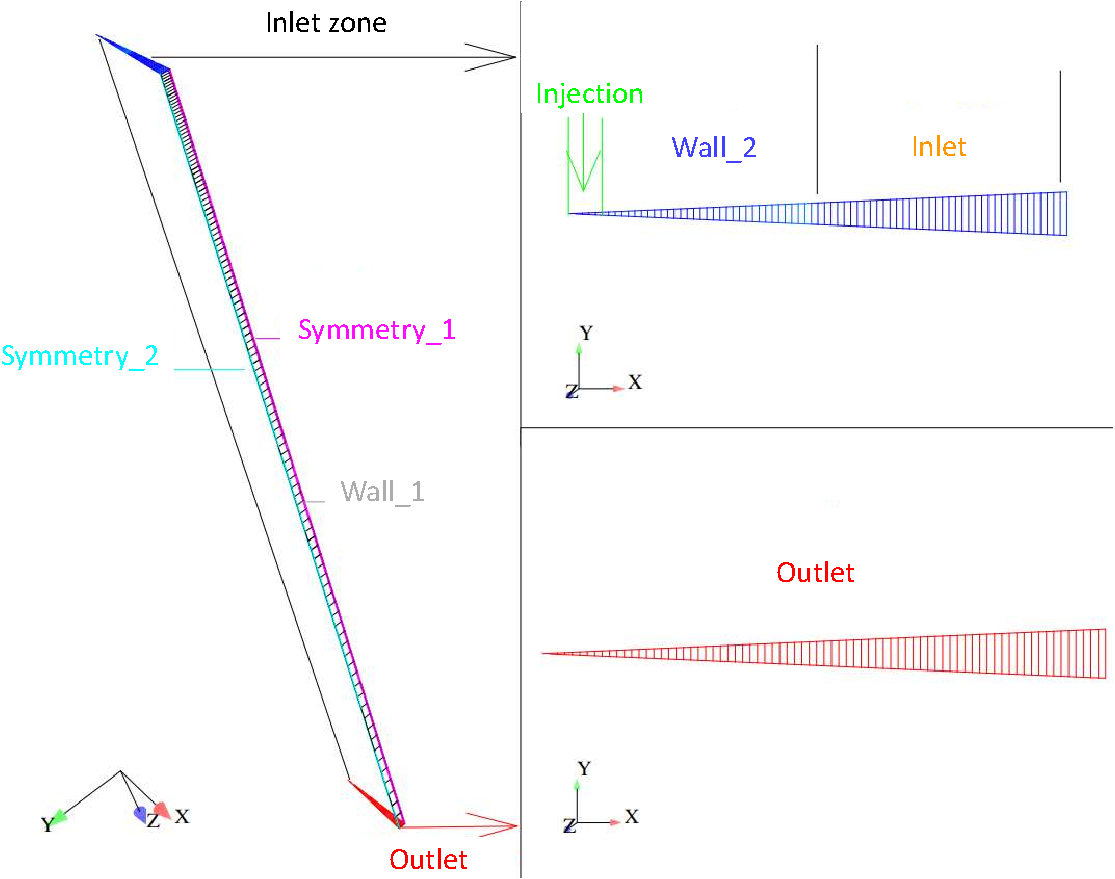
\includegraphics[width=12cm]{\IMAGES/BC_graph.pdf}}
   \caption{\label{couleur}{Names of the boundary conditions}}
\end{figure}

\item[$\bullet$] \textbf{Particles inlet data}:

The injection data of the particle cloud taken from the experimental data are listed in table \ref{CL_part}. One may note that the fluctuations in radial and tangential velocity are identical.

\begin{table}[H]
   \begin{center}
      \begin{tabular}{|c|c|c|c|c|c|c|} \hline
         Coordinate  & Velocity    & Velocity    & Velocity   &
         Fluctuation & Fluctuation & Fluctuation                                               \\
         radial      & axial       & radial      & tangential & velocity
                     & velocity    & velocity                                                  \\
                     & mean        & mean        & mean       & axial
                     & radial      & tangential                                                \\
         $mm$        & $m/s$       & $m/s$       & $m/s$      & $m/s$    & $m/s$    & $m/s$    \\ \hline
         0           & 3,989888    & 0,021573    & 0          & 0,492889 & 0,145902 & 0,145902 \\ \hline
         2           & 3,955918    & 0,019587    & 0          & 0,248873 & 0,153009 & 0,153009 \\ \hline
         4           & 3,818365    & 0,019053    & 0          & 0,276544 & 0,161393 & 0,161393 \\ \hline
         6           & 3,615492    & 0,018448    & 0          & 0,339334 & 0,174045 & 0,174045 \\ \hline
         8           & 3,235091    & 0,015862    & 0          & 0,45922  & 0,232101 & 0,232101 \\ \hline
         10          & 2,148246    & 0,098097    & 0          & 0,60341  & 0,198226 & 0,198226 \\ \hline
      \end{tabular}
   \end{center}
   \caption{Dispersed phase distribution profiles.}
   \label{CL_part}
\end{table}

The instantaneous velocity of the particles is calculated based on the mean velocity components and the velocity fluctuations $\mathbf{u_p}=(u_p,v_p,w_p)$. For each particle, an injection point is picked randomly in the injection plane. Depending on the injection point radius, the mean and fluctuation velocity components of the particle are first computed in the cylindrical coordinates system. The instantaneous velocity is then calculated based on drawing three random variables, $\eta_1$, $\eta_2$ et $\eta_3$ following a normal distribution. The instantaneous particle velocity may then be calculated in the cylindrical coordinate system.
\begin{equation}
   \left\{\begin{array}{l}
      {u_p}_r=<{u_p}_r>+\eta_1 {u_p}_r^\prime \\
      {u_p}_\theta=\eta_2{u_p}_{\theta}^\prime\qquad\qquad\qquad
      \text{(${u_p}_\theta=0$)}               \\
      {u_p}_z=<{u_p}_z>+\eta_3{u_p}_z^\prime  \\
   \end{array}\right.
\end{equation}

The velocity is then converted to the mesh's Cartesian coordinate system:
\begin{equation}
   \left\{\begin{array}{l}
      u_p=cos\theta\, {u_p}_r- sin\theta\, {u_p}_\theta \\
      v_p=sin\theta\, {u_p}_r+ cos\theta\, {u_p}_\theta
   \end{array}\right.
\end{equation}

Similarly, the instantaneous fluid velocity is obtained from the experimental data in table \ref{CL_fluide}: interpolation of the fluid velocity mean and fluctuating components at the cell centre, reconstruction of the instantaneous velocity, and conversion to the mesh's Cartesian coordinate system \footnote{By default, during the injection phase \CS\ uses the continuous phase's mean velocity as the fluid velocity which is seen by the particles. For this work, we have used the instantaneous fluid velocity.}.

\noindent
The particle injection mass flow rate is $1~kg/h$. For the reduced, axisymmetric domain, this translates to $0,385.10^{-5}~kg/s$.,This is equivalent to injecting $13.8$ particles per time step in the computational domain, for $60~\mu m$ diameter particles and a $0,001~s$ time step. However, given the distribution of particle diameters, we chose to inject only $10$ particles per time step. The statistical weight of each particle is then adjusted with regard to the mass flow rate.\\

\item[$\bullet$] \textbf{Particle boundary conditions} :
%
\begin{table}[H]
   \begin{center}
      \begin{tabular}{lccc}
         \hline\hline
            BC & Name & Particle boundary conditions           \\      
         \hline
         BC\_1 & Injection 	& inlet \\
         BC\_2 & Inlet 	& outlet \\
         BC\_3 & Outlet	& outlet \\
         BC\_4 & Symmetry-1 	& perfect rebound \\
         BC\_5 & Symmetry-2 	& perfect rebound \\
         BC\_6 & Wall-1 	& perfect rebound \\
         BC\_7 & Wall-2 	& perfect rebound \\
         \hline\hline
      \end{tabular}
   \end{center}
\end{table}
%

\item[$\bullet$] \textbf{Fluid boundary conditions} :

\begin{table}[H]
   \begin{center}
      \begin{tabular}{lccc}
         \hline\hline
            BC & Name & Fluid boundary conditions  \\      
         \hline
         BC\_1 & Injection 	& inlet \\
         BC\_2 & Inlet 	& inlet \\
         BC\_3 & Outlet	& outlet \\
         BC\_4 & Symmetry-1 	& symmetry \\
         BC\_5 & Symmetry-2 	& symmetry \\
         BC\_6 & Wall-1 	& wall	 \\
         BC\_7 & Wall-2 	& wall	 \\
         \hline\hline
      \end{tabular}
   \end{center}
\end{table}

\begin{description}
\item[-] \textbf{Inlet} : Dirichlet condition on the mean velocity components, the distribution profiles from the experiments are listed in table \ref{CL_fluide}. The second component of the mean velocity, $<v>$, is nought. \footnote{Although the experimental data is listed in a cylindrical reference frame, it is trivial to convert it in the Cartesian frame of the mesh since the two reference frames are aligned on the latter's axes.}. One may note that the fluctuations in radial and tangential velocity are identical.

\begin{table}[H]
\begin{center}
\begin{tabular}{|c|c|c|c|c|c|c|} \hline
Coordinate  & Velocity  & Velocity  & Velocity &
Fluctuation  & Fluctuation  & Fluctuation  \\
radial  & axial    &   radial  &  tangential   & velocity
& velocity    & velocity   \\
&mean & mean  & mean &  axial
&    radial &  tangential  \\
$mm$   & $m/s$  &  $m/s$ & $m/s$ & $m/s$& $m/s$& $m/s$ \\  \hline
0    & 3,989888 &  0,043071 & 0  & 0,2206   & 0,165755 & 0,165755 \\   \hline
2    & 3,955918 &  0,056412 & 0  & 0,235237 & 0,167099 & 0,167099 \\   \hline
4    & 3,818365 &  0,071609 & 0  & 0,280546 & 0,188935 & 0,188935 \\   \hline
6    & 3,615492 &  0,056304 & 0  & 0,345076 & 0,196318 & 0,196318 \\   \hline
8    & 3,235091 &  0,067233 & 0  & 0,480505 & 0,199175 & 0,199175 \\   \hline
10    & 1,15302  &  0,057133 & 0  & 0,462576 & 0,192527 & 0,192527 \\   \hline
76    & 4,609382 & -0,078698 & 0  & 0,620767 & 0,297634 & 0,297634 \\   \hline
80    & 5,050922 & -0,062107 & 0  & 0,412637 & 0,26486  & 0,26486  \\   \hline
84    & 5,349239 & -0,043911 & 0  & 0,378357 & 0,253143 & 0,253143 \\   \hline
88    & 5,663382 & -0,060412 & 0  & 0,33724  & 0,227446 & 0,227446 \\   \hline
92    & 5,774033 & -0,039152 & 0  & 0,309257 & 0,198263 & 0,198263 \\   \hline
96    & 5,852311 & -0,041603 & 0  & 0,268617 & 0,180068 & 0,180068 \\   \hline
100    & 5,957135 & -0,047923 & 0  & 0,26992  & 0,16104  & 0,16104  \\   \hline
104    & 6,0781   & -0,034075 & 0  & 0,248661 & 0,157479 & 0,157479 \\   \hline
108    & 6,075214 & -0,043817 & 0  & 0,239869 & 0,145587 & 0,145587 \\   \hline
112    & 5,910082 & -0,028827 & 0  & 0,24758  & 0,16021  & 0,16021  \\   \hline
116    & 5,932579 & -0,029241 & 0  & 0,238192 & 0,15885  & 0,15885  \\   \hline
120    & 5,929479 & -0,015086 & 0  & 0,31793  & 0,186978 & 0,186978 \\   \hline
124    & 5,824071 &  0,017707 & 0  & 0,337416 & 0,201831 & 0,201831 \\   \hline
127    & 5,773876 &  0,045791 & 0  & 0,338541 & 0,214657 & 0,214657 \\   \hline
\end {tabular}
\end{center}
\caption{Continuous phase profiles.}
\label{CL_fluide}
\end{table}

\item[-]\textbf{Free outlet}: zero flux, homogeneous Neumann condition.

\item[-]\textbf{Wall}: friction condition (two velocity scale wall model).

\item[-]\textbf{Symmetry}: symmetry.

\item[-]\textbf{Initial conditions} : $<u>=0~;~<v>=0~;~<w>=0$.

\end{description}

\item[$\bullet$] \textbf{Pressure boundary conditions} :
\begin{description}
   \item[-]\textbf{Inlet}: Homogeneous Neumann.
   \item[-]\textbf{Free outlet}: Standard condition.
   \item[-]\textbf{Wall}: Homogeneous Neumann.
   \item[-]\textbf{Symmetry}: Homogeneous Neumann.
\end{description}

\item[$\bullet$] \textbf{"Reynolds tensor" and "Turbulent dissipation" boundary conditions} :

\begin{description}
   \item[-]\textbf{Inlet}: Dirichlet condition. Given that only the velocity fluctuations are known, it is not possible to recalculated the cross-components of the Reynolds tensor. However, initialising only the diagonal to non-zero values using the measured fluctuating values whilst leaving the cross-components null leads to wrong results. Instead, it is necessary to use the turbulent kinetic energy to initialise the diagonal components and leave the cross-components at zero.

         \begin{description}

            \item[$\rightarrow$] Kinetic turbulent energy from the experimental data:
                  \begin{displaymath}
                     k_{ent} = \frac{1}{2} \left( <{u'}^2> + <{v'}^2> + <{w'}^2> \right)
                  \end{displaymath}

            \item[$\rightarrow$] Reynolds tensor diagonal components:
                  \begin{displaymath}
                     R_{ii} = \frac{2}{3} k_{ent}
                  \end{displaymath}

            \item[$\rightarrow$] Reynolds tensor cross-components:
                  \begin{displaymath}
                     R_{ij} = 0
                  \end{displaymath}

            \item[$\rightarrow$] Turbulent dissipation based on the method programmed in \textbf{cs\_user\_boundary\_conditions.f90} and in \textbf{cs\_user\_modules.f90}:
                  \begin{description}
                     \item[+] Primary inlet hydraulic diameter: $D_h=0,02~m$
                     \item[+] Secondary inlet hydraulic diameter: $D_h=0,15~m$
                     \item[+] The Reynolds number
                           $\displaystyle{R_e=\frac{D_h V}{\nu}}$ makes it possible to calculate the friction velocity, $u^*$, using the following formula:
                           \begin{displaymath}
                              u^* = V \sqrt{\frac{\lambda}{8}} \quad \text{avec} \quad
                              \begin{cases}
                                 \displaystyle
                                 \lambda = 0,3164 Re^{-0,25} & \text{si} \; Re \leq 30000 \\
                                 \lambda = 0,184 Re^{-0,2}   & \text{si} \; Re \geq 30000
                              \end{cases}
                           \end{displaymath}
                     \item[+] Inlet turbulent dissipation:
                           \begin{displaymath}
                              \varepsilon_{ent} = C_{\mu} \frac{{k_{ent}}^2}{\kappa \, u^* \, 0,1 \, D_h}
                           \end{displaymath}
                           where $C_{\mu}=0,09$ and $\kappa=0,41$ (constant of K\'arm\'an).
                  \end{description}

         \end{description}

   \item[-]\textbf{Free outlet}: Homogeneous Neumann.
   \item[-]\textbf{Wall}: Turbulent wall model.
   \item[-]\textbf{Symmetry plane}: Homogeneous Neumann. 

   \item[-]\textbf{Initial conditions} : Automatically set based on $U_{ref}=1~m/s$.
\end{description}

\end{itemize}

\subsection{Numerical schemes}


\subsection{User coding}

\begin{description}

   \item[-] \textbf{cs\_user\_modules.f90} : programs to interpolate the experimental data at the inlet.
   
   \item[-] \textbf{cs\_user\_boundary\_conditions.f90} : definition of the continuous phase boundary conditions as a function of the border faces
   
   \item[-] \textbf{cs\_user\_lagr\_particle.c} : definition of the dispersed phase boundary conditions as a function of the border faces
   
   \item[-] \textbf{cs\_user\_extra\_operations.f90} : clipping the $\varepsilon$ field during the two-way coupling calculation with the complete model with the local rotation option to help the code to run.

\end{description}

\subsection{Calculation strategy}

The runs are carried out in two steps. The first step is a single phase calculation, without particles. This makes it possible to initialise the two-phase calculation or the Langevin calculation.\\ 

\begin{description}

   \item[$\bullet$]\textbf{Single phase calculation}
         \begin{itemize}
            \item[-] {\bf Restart:} NO
            \item[-] {\bf Total number of time steps:} 2000 ($2~s$)
            \item[-] {\bf Time step: constant (\texttt{IDTVAR=0}), } $10^{-3}~s$
         \end{itemize}


   \item[$\bullet$]\textbf{Complete two-phase calculation}
         \begin{itemize}
            \item[-] {\bf Restart:} YES
            \item[-] {\bf Restart of the Lagrangian calculation:} NO
            \item[-] {\bf Total number of additional time steps:} 5000 ($7~s$)
                  (i.e. the number of Lagrangian steps)
            \item[-] {\bf Time step: (\texttt{IDTVAR=0}),} $10^{-3}~s$
            \item[-] \textbf{Stationary continuous phase:} YES (\texttt{ISTTIO=1})

            \item[-] {\bf Turbulent dispersion model:}
                  \begin{itemize}
                     \item[*] For the two-phase calculation, the default complete modele with the local rotation

                  \end{itemize}
            \item[-] {\bf Dynamic two-way coupling:} YES (\texttt{IILAGR=2} and \texttt{LTSDYN=1})
            \item[-] {\bf Time averaging of the two-way coupling terms:} YES, starting from Lagrangian step 1500 ($3.5~s$) (\texttt{NSTITS=1500}); figure
                  \ref{nbpart} shows that the particle loading in the calculation domain may be considered as complete by that step
            \item[-] {\bf Calculation of volumetric statistics:} YES

                  (\texttt{IDSTNT=1}) activate the calculation of the volumetric statistics

            \item[-] {\bf Time averaging of the volumetric statistics:} YES, starting at Lagrangian 2000 ($4~s$) (\texttt{NSTIST=2000}); figure \ref{nbpart} indicates that this is reasonable.
            \item[-] {\bf Total number of particles injected at each time step:} 10
         \end{itemize}
         
   \item[$\bullet$]\textbf{Langevin calculation}
         \begin{itemize}
            \item[-] {\bf Restart:} YES
            \item[-] {\bf Restart of the Lagrangian calculation:} NO
            \item[-] {\bf Total number of additional time steps:} 5000 ($7~s$)
                  (i.e. the number of Lagrangian steps)
            \item[-] {\bf Time step: (\texttt{IDTVAR=0}),} $10^{-3}~s$
            \item[-] \textbf{Stationary continuous phase:} YES (\texttt{ISTTIO=1})
            \item[-] {\bf Dynamic one-way coupling:} YES (\texttt{IILAGR=1} and \texttt{LTSDYN=1})
            \item[-] {\bf Fluid-like tracer particles:} YES
            \item[-] {\bf Calculation of volumetric statistics:} YES
                  (\texttt{IDSTNT=1}) activate the calculation of the volumetric statistics
            \item[-] {\bf Time averaging of the volumetric statistics:} YES, starting at Lagrangian 2000 ($4~s$) (\texttt{NSTIST=2000}); figure \ref{nbpart} indicates that this is reasonable.
            \item[-] {\bf Total number of particles injected at each time step:} 10
         \end{itemize}

For the the two-way coupling calculation with the complete model with the local rotation option, the field "$\varepsilon$" were hardly clipped to keep the calculation running. If the coupling source terms are time averaged from the first lagrangian iteration, the code is more stable. The code become hardly instable when the time average of coupling source term starts when the number of particles in the domain is constant (around 3.5s) that it is done in the present study.


\end{description}

% =============================
\section{Results}
% =============================

\subsection{Run data}

\begin{description}

   \item[$\bullet$]\textbf{Single phase run}

         \begin{itemize}
            \item[$\bullet$] Inlet flow at the outlet: NO
            \item[$\bullet$] Number of clips on $R_{ij}-\varepsilon$ in the listing: none
            \item[$\bullet$] Maximum CFL number of the order of 1.75 (very stable)
         \end{itemize}

   \item[$\bullet$]\textbf{"complete" two-phase run}

         \begin{itemize}
            \item[$\bullet$] Inlet flow at the outlet: NO
            \item[$\bullet$] Number of clips on $R_{ij}-\varepsilon$ in the listing: none
            \item[$\bullet$] Maximum CFL number of the order of 1.75 (very stable)
            \item[$\bullet$] Percentage of lost particles: $0,0$\%
         \end{itemize}
         
   \item[$\bullet$]\textbf{"Langevin" run}

         \begin{itemize}
            \item[$\bullet$] Inlet flow at the outlet: NO
            \item[$\bullet$] Number of clips on $R_{ij}-\varepsilon$ in the listing: none
            \item[$\bullet$] Maximum CFL number of the order of 1.75 (very stable)
            \item[$\bullet$] Percentage of lost particles: $0,0$\%
         \end{itemize}

   \item[$\bullet$]\textbf{Single phase run convergence}

         Figure \ref{Histo_mono} shows the time history of the axial and radial components of the mean velocity, the diagonal terms of the Reynolds tensor, and the turbulent dissipation recorded at 15 different points (table \ref{tab_capteur} and figure \ref{pospoints})

         \begin{table}[H]
            \begin{center}
               \begin{tabular}{|c|c|c|c|}
                  \hline
                  $Probe$ & $Probe~number$ & $X$ & $Z$ \\
                  \hline
                  $A$ & $1$ & $0,02$ & $0,89.10^{-2}$ \\
                  \hline
                  $B$ & $2$ & $0,02$ & $0,49.10^{-1}$ \\
                  \hline
                  $C$ & $3$ & $0,02$ & $0,25$         \\
                  \hline
                  $D$ & $4$ & $0,02$ & $0,5$          \\
                  \hline
                  $E$ & $5$ & $0,02$ & $1$            \\
                  \hline
                  $F$ & $6$ & $0,07$ & $0,89.10^{-2}$ \\
                  \hline
                  $G$ & $7$ & $0,07$ & $0,49.10^{-2}$ \\
                  \hline
                  $H$ & $8$ & $0,07$ & $0,25$         \\
                  \hline
                  $I$ & $9$ & $0,07$ & $0,5$          \\
                  \hline
                  $J$ & $10$ & $0,07$ & $1$            \\
                  \hline
                  $K$ & $11$ & $0,12$ & $0,89.10^{-2}$ \\
                  \hline
                  $L$ & $12$ & $0,12$ & $0,49.10^{-1}$ \\
                  \hline
                  $M$ & $13$ & $0,12$ & $0,25$         \\
                  \hline
                  $N$ & $14$ & $0,12$ & $0,5$          \\
                  \hline
                  $P$ & $15$ & $0,12$ & $1$            \\
                  \hline
               \end{tabular}
               \caption{Probe coordinates ($m$)}
               \label{tab_capteur}
            \end{center}
         \end{table}

         \begin{figure}[H]
            \centerline{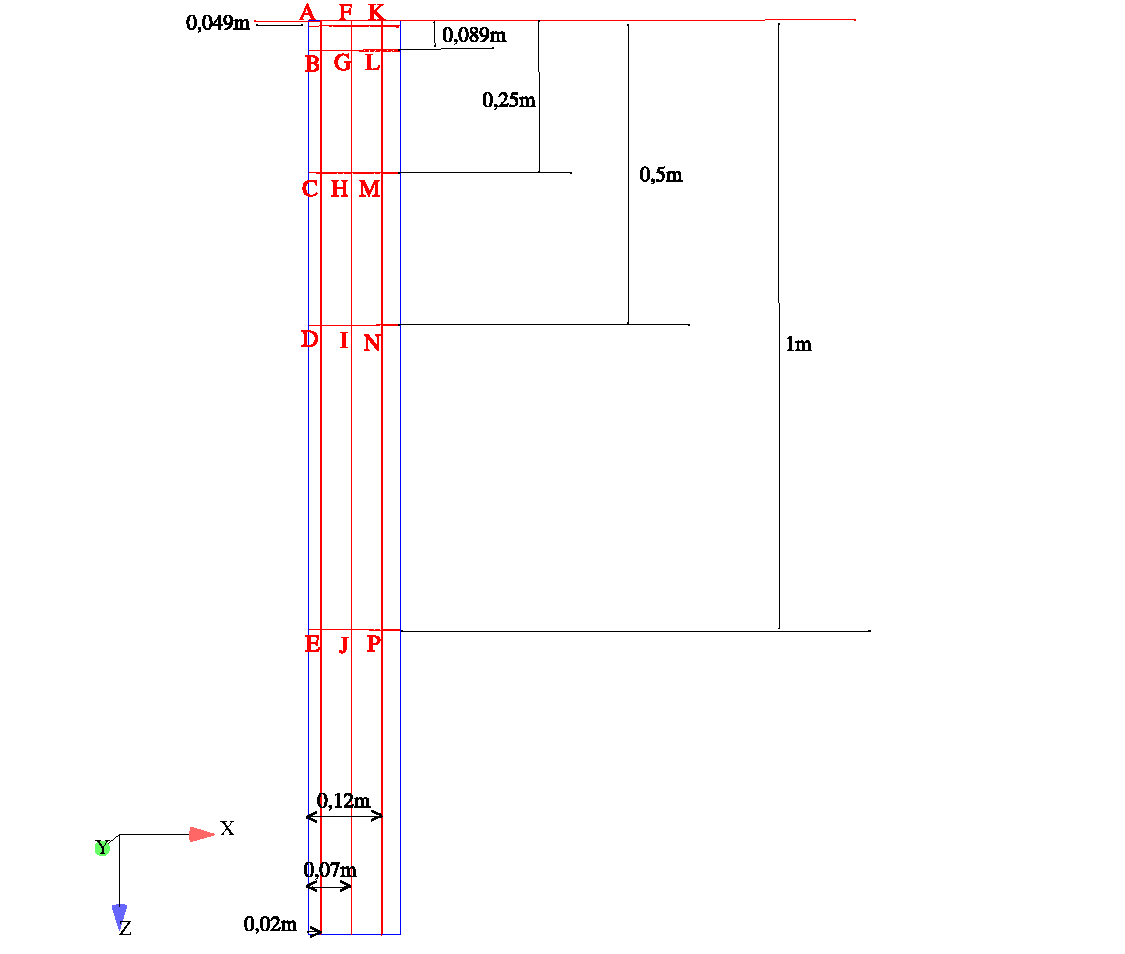
\includegraphics[width=15.cm]{\IMAGES/pospoints-eps-converted-to.pdf}}
            \caption{Probe locations.}
            \label{pospoints}
         \end{figure}

         \begin{figure}[H]
            \centerline{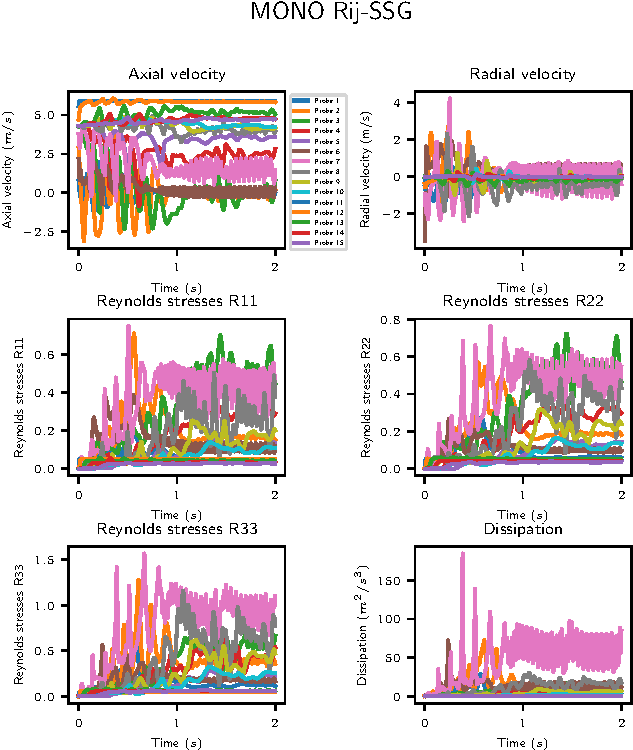
\includegraphics[width=14.cm]{\IMAGES/VNV/probes_MONO-RijSSG.pdf}}
            \caption{Single phase calculation: convergence history of the axial and radial mean velocity components, Reynolds stresses $R_{11}$, $R_{22}$, $R_{33}$ and the dissipation.}
            \label{Histo_mono}
         \end{figure}

         Globally, the graphs show that the calculations are converged within the 2000 iterations. Although, probes F (probe number 6) and G (probe number 7) display oscillations around a mean value. This can be explained by the probes' position just upstream of the separation of the two inlets in the recirculation zone. As the oscillations are stable, the run is considered converged.

   \item[$\bullet$]\textbf{Two-phase run convergence}

         For the two-phase run, the figure \ref{Histo_Cplt} show the time histories of the continuous phase mean velocity axial and radial components, the Reynolds stresses $R_{11}$, $R_{22}$, $R_{33}$ and the
         dissipation. As for the single phase calculation, probes F (probe number 6) and G (probe number 7) display oscillations around a mean value.
         The graphs indicate that the two-phase runs may be considered converged by time step $3.5~s$.


         \begin{figure}[H]
            \centerline{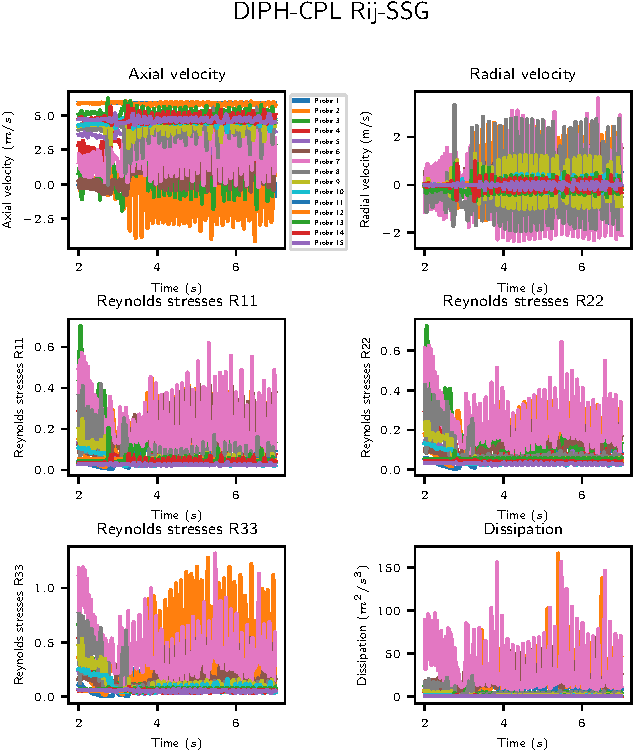
\includegraphics[width=14.cm]{\IMAGES/VNV/probes_DIPH-CPL-RijSSG.pdf}}
            \caption{"complete" two-phase run: convergence history of the mean velocity axial and radial components, the Reynolds stresses $R_{11}$, $R_{22}$, $R_{33}$ and the dissipation.}
            \label{Histo_Cplt}
         \end{figure}

   \item[$\bullet$]\textbf{Langevin run convergence}

         For the Langevin run, the figures \ref{Histo_Lang} show the time histories of the continuous phase mean velocity axial and radial components, the Reynolds stresses $R_{11}$, $R_{22}$, $R_{33}$ and the
         dissipation. As for the single phase calculation, probes F (probe number 6) and G (probe number 7) display oscillations around a mean value.
         The graphs indicate that the Langevin run may be considered converged by time step $3.5~s$.


         \begin{figure}[H]
            \centerline{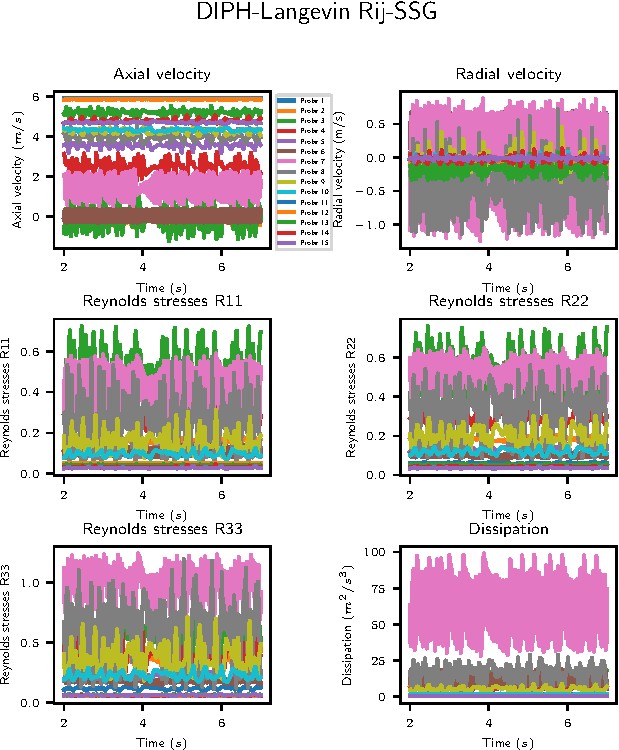
\includegraphics[width=14.cm]{\IMAGES/VNV/probes_DIPH-Langevin-RijSSG.pdf}}
            \caption{"Langevin" run: convergence history of the mean velocity axial and radial components, the Reynolds stresses $R_{11}$, $R_{22}$, $R_{33}$ and the dissipation.}
            \label{Histo_Lang} 
         \end{figure}


   \item[$\bullet$] \textbf{Total number of particles in the computational domain}

         Figure \ref{nbpart} shows the time history of the total number of particles in the computational domain for both two-phase runs. The number of particles stabilises $3.5~s$. \\ The maximum number of particles obtained in the two runs is different, of the order of $4500$ particles in the "complete" two-phase run compared to about $9000$ for the "Langevin" run.\\

         \begin{figure}[H]
            \centerline{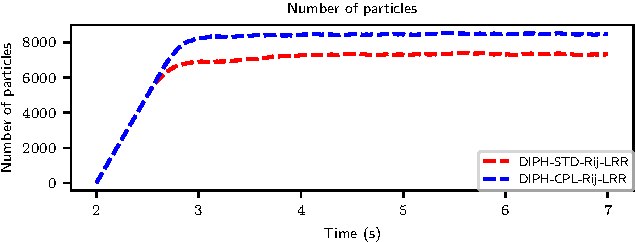
\includegraphics[width=9cm]{\IMAGES/VNV/Number_of_particles.pdf}}
            \caption{Time evolution of the total number of particles in the computational domain.}
            \label{nbpart}
         \end{figure}

\end{description}

\clearpage

\subsection{Comparisons between experimental and computed values}

\subsubsection{Single-phase run}

The measured and computed mean velocity axial components are compared along the $z$ axis in figure \ref{AxeFluide_mono} and along horizontal plane sections at $z = 0,003~m$, $0,08~m$, $0,16~m$, $0,24~m$, $0,32~m$, $0,42~m$ in \ref{ProfVZFluide_mono}. On these graphs, the velocity fields are time averaged from $t=1.5~s$ to $2~s$.

\begin{figure}[H]
   \centerline{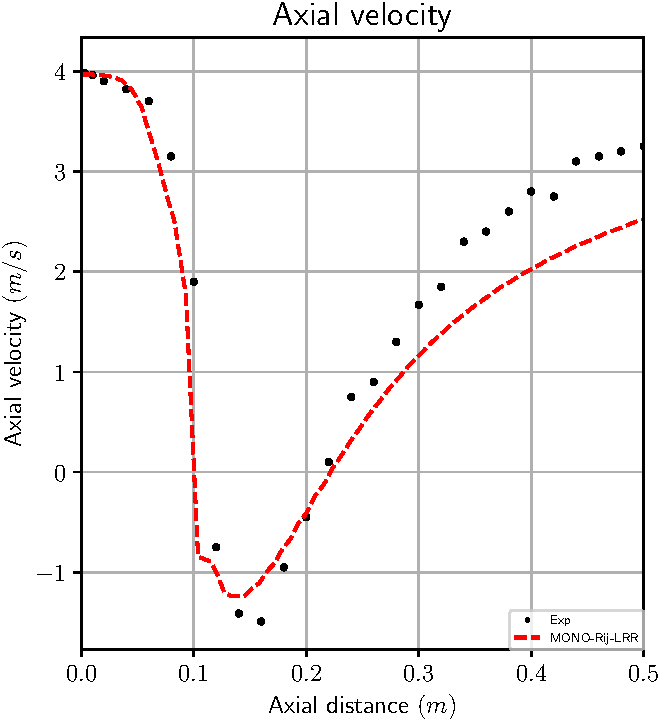
\includegraphics[width=13cm]{\IMAGES/VNV/Axial_profile_MONO.pdf}}
   \caption{Single phase run: fluid mean velocity axial component along the centre line.}
   \label{AxeFluide_mono}
\end{figure}

\noindent
Looking at the graph, the flow is divided in three large regions which are separated by the two stagnation points around $0.1m$ and $0.2m$ on figure \ref{AxeFluide_mono} and named $S_{1}$ and $S_{2}$ on figure \ref{ecoulement}. The first region, (called A on figure \ref{ecoulement}) situated between the primary inlet and the first stagnation point is representative of the central jet penetration. The calculation gives a reasonable prediction for an axial distance inferior to $0.15m$. The second region (called B on figure \ref{ecoulement}), located between the two stagnation points represents the recirculation zone. The calculation doesn't give a good prediction, particularly with regard to the position of points $S_{1}$ and $S_{2}$. The minimum velocity is slightly underestimated. The third zone (called C on figure \ref{ecoulement}) denotes the zone where the annular flow reaches the axis of symmetry and evolves towards a free jet flow. The results from the run are offset from the experimental results in this zone. Whilst the offset is also evident on the radial profiles at $z=0,32~m$ and $z=0,42~m$ in figure \ref{ProfVZFluide_mono}, it is smaller. In any case, according to \cite{Rap3}, there are reasons to question the experimental measurements in this region.

\begin{figure}[H]
   \centerline{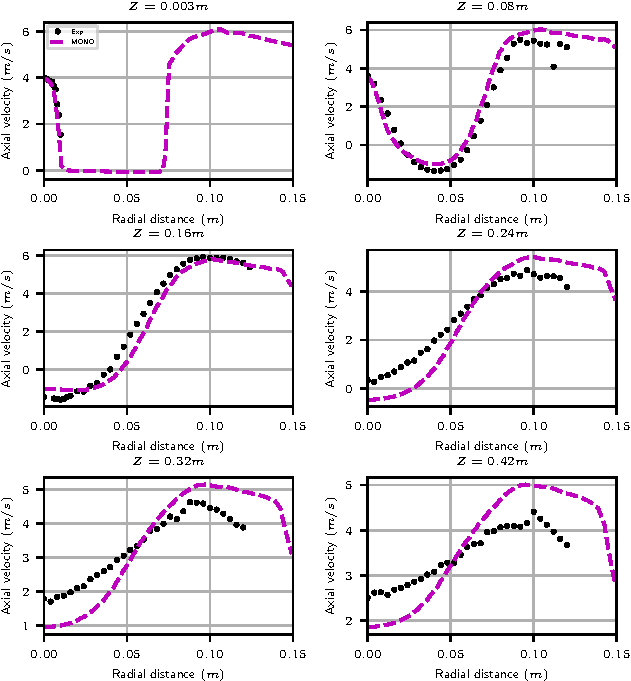
\includegraphics[width=14cm]{\IMAGES/VNV/Radial_profile_MONO.pdf}}
   \caption{Single-phase run: fluid mean velocity axial component profiles at the different measurement plane sections.}
   \label{ProfVZFluide_mono}
\end{figure}

\clearpage

\subsubsection{Two-phase and Langevin runs}

\begin{description}
   \item[$\bullet$] \textbf{Continuous phase} :
\end{description}

Figures \ref{AxeFluide_diph} and \ref{ProfVZFluide_diph} show the calculated continuous phase mean velocity axial component. As for the single-phase run, the fluid and particle velocity fields are time averaged from $t=4~s$ to $7~s$. Figure \ref{AxeFluide_diph} shows the profiles along the centre line, $z$, whereas figure \ref{ProfVZFluide_diph} shows the profiles along the plane sections at $z = 0,003~m$, $0,08~m$, $0,16~m$, $0,24~m$, $0,32~m$, $0,42~m$.

\noindent

The continuous phase flow predictions do not differ much between the single phase run and the "Langevin" run but differ a lot between the single-phase and the "complete" two-phase run. The figure \ref{AxeFluide_diph} indicates that the "complete" two-phase run do not give correct predictions of the first two zones: the penetration length of the primary inlet jet is underestimated and the length of the recirculation zone between the two stagnation points is shorter. The comparisons in the transversal plane sections show that the difference between the measured and computed values is significant mostly in a zone very close to the centre line. Figure \ref{ProfVZFluide_diph} shows as well that the quality of the predicted values deteriorates with distance from the inlets.

\begin{figure}[H]
   \centerline{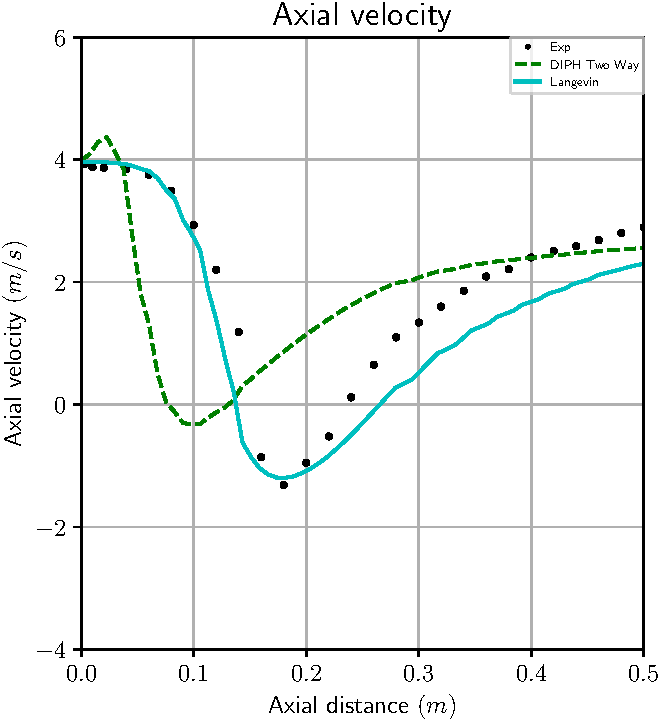
\includegraphics[width=13cm]{\IMAGES/VNV/Axial_profile_DIPH.pdf}}
   \caption{"Complete" two-phase and "Langevin" runs: mean fluid velocity axial component along the centre line.}
   \label{AxeFluide_diph}
\end{figure}

\begin{figure}[H]
   \centerline{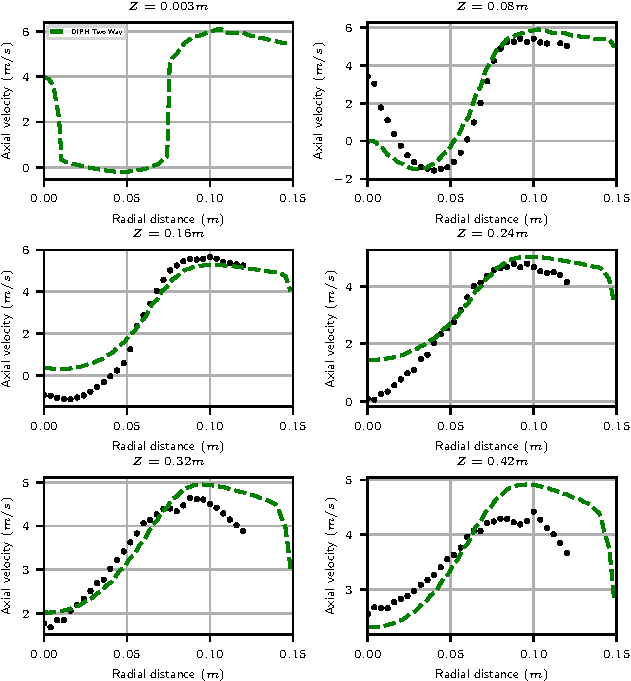
\includegraphics[width=14cm]{\IMAGES/VNV/Radial_profile_DIPH.pdf}}
   \caption{"Complete" two-phase and "Langevin" runs: mean fluid velocity axial component profiles along the different measurement planes.}
   \label{ProfVZFluide_diph}
\end{figure}

\begin{description}
   \item[$\bullet$] \textbf{Dispersed phase} :
\end{description}
\noindent

The calculated mean dispersed phase velocity axial and radial components are shown in figures \ref{VitZPart} and \ref{VitXPart} along the plane sections at $z = 0,003~m$, $0,08~m$, $0,16~m$, $0,24~m$, $0,32~m$, and $0,42~m$.
Figures \ref{VitZpPart} et \ref{VitXpPart} show the fluctuation dispersed phase velocity axial and radial components.

\noindent
Away from the external edges of the particle cloud (near the edges of the measuring points), the calculated mean axial velocities are in acceptable agreement with the experimental ones. However, the results for the mean radial velocity are more questionable. \\ With regard to the axial or radial component of the fluctuating particle velocity, the "complete" or the "Langevin" run show poor predictions.

\noindent

\begin{figure}[H]
   \centerline{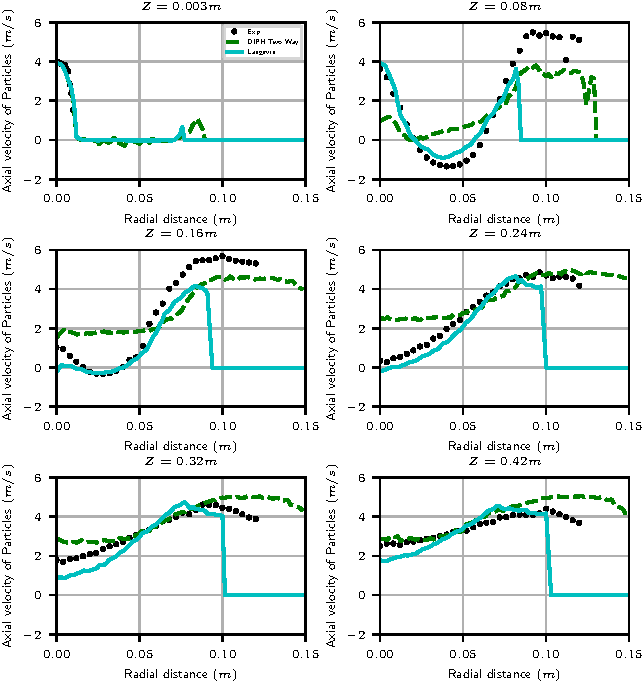
\includegraphics[width=14cm]{\IMAGES/VNV/Radial_profile_mean_axial_vel_part_DIPH.pdf}}
   \caption{Two-phase run: profiles of the mean particle velocity axial component along the different measurement plane sections.}
   \label{VitZPart}
\end{figure}

\begin{figure}[H]
   \centerline{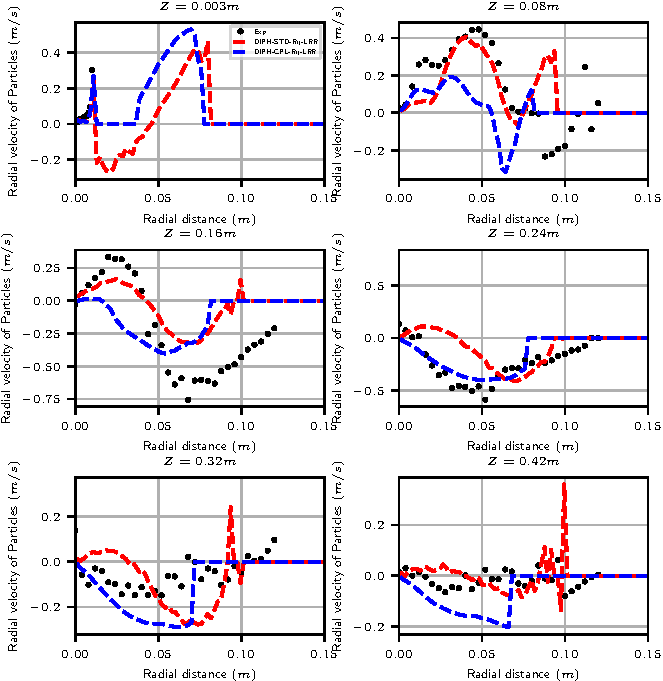
\includegraphics[width=14cm]{\IMAGES/VNV/Radial_profile_mean_radial_vel_part_DIPH.pdf}}
   \caption{Two-phase run: profiles of the mean particle velocity radial component along the different measurement plane sections.}
   \label{VitXPart}
\end{figure}

\begin{figure}[H]
   \centerline{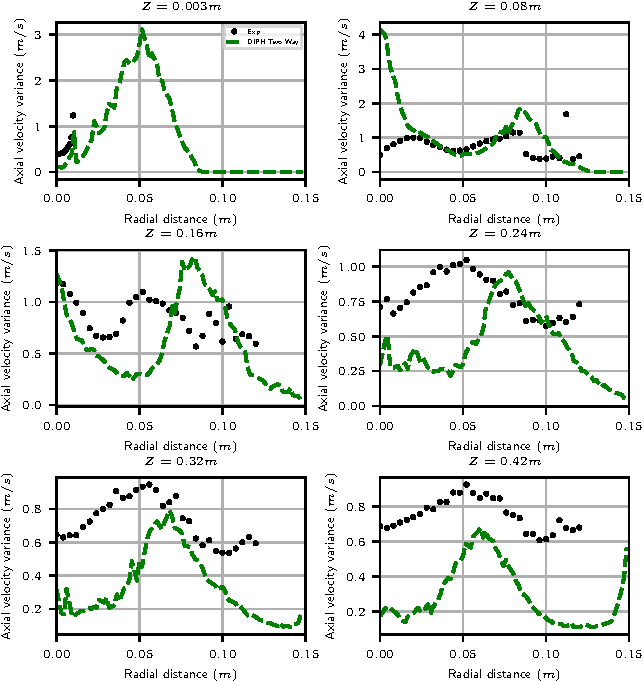
\includegraphics[width=14cm]{\IMAGES/VNV/Radial_profile_mean_axial_flu_vel_part_DIPH.pdf}}
   \caption{Two-phase run: profiles of the fluctuating particle velocity axial component along the different measurement plane sections.}
   \label{VitZpPart}
\end{figure}

\begin{figure}[H]
   \centerline{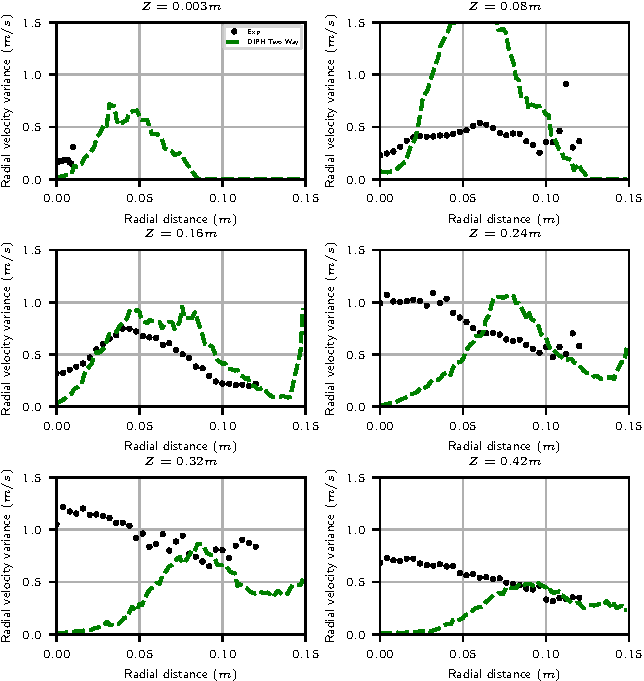
\includegraphics[width=14cm]{\IMAGES/VNV/Radial_profile_mean_radial_flu_vel_part_DIPH.pdf}}
   \caption{Two-phase run: profiles of the fluctuating particle velocity radial component along the different measurement plane sections.}
   \label{VitXpPart}
\end{figure}

\clearpage

\section{Archiving}

The directory for the case is named: \textbf{HERCULE}

The sub-directories are organised as follows:
\medskip\\
\hspace*{2cm}\textbf{HERCULE-MONO-RijSSG}: everything having to do with the single-phase calculation.
\medskip\\
\hspace*{2cm}\textbf{HERCULE-DIPH-Langevin-RijSSG}: everything having to do with the "Langevin" calculation.
\medskip\\
\hspace*{2cm}\textbf{HERCULE-DIPH-CPL-RijSSG}: everything having to do with the "complete" two-phase calculation.



